\documentclass[a4paper,12pt,twoside]{article}
\usepackage{graphicx}
\graphicspath{ {./images/} }
\usepackage{wrapfig}
%\usepackage{indentfirst} % Uncomment to indent first paragaph of each section (not really correct for academic papers, but follows more common business convention)

\usepackage{geometry}
\geometry{
  a4paper,
  total={170mm,257mm},
  left=20mm,
  top=40mm,
  bottom=30mm,
}

\usepackage{fontspec}
\setmainfont{Exo 2}[%
    Path            =   fonts/,
    Extension       =   .otf,
    UprightFont     =   *-Regular,
    ItalicFont      =   *-Italic,
    BoldFont        =   *-Bold,
    BoldItalicFont  =   *-BoldItalic,
    FontFace        =   {black}{n}{*-Black},
    FontFace        =   {black}{it}{*-BlackItalic},
]

\usepackage[dvipsnames]{xcolor}
\definecolor{RHgrey}{RGB}{101,101,101}
\definecolor{RHblue}{RGB}{7,163,216}
\definecolor{RHgreen}{RGB}{30,165,43}
\definecolor{RHyellow}{RGB}{251,210,0}
\definecolor{code}{RGB}{200,200,200}
  
\usepackage{sectsty}
\sectionfont{\color{RHblue}} 
\subsectionfont{\color{RHblue}}
\subsubsectionfont{\color{RHblue}}

\usepackage[utf8]{inputenc}
\usepackage[english]{babel}

\usepackage{multicol} % Allows multiple columns to be used on the fly

\usepackage{fancyhdr}
\pagestyle{fancy}
\fancyhf{}
\lhead{\color{RHgrey} \leftmark}
\rhead{\color{RHgrey} \rightmark}
\fancyfoot[LE]{\color{RHgrey} \thepage \hspace{5mm} \scriptsize RAMANI HURIA INTERIM REPORT 4}
\fancyfoot[RO]{\color{RHgrey} \scriptsize RAMANI HURIA INTERIM REPORT 4 \hspace{3mm} \normalsize \thepage}

\usepackage{hyperref}
\hypersetup{
  colorlinks=true,
  linkcolor=RHblue, % to match the Ramani Huria blue text
  filecolor=magenta,      
  urlcolor=cyan,
  pdftitle={RH Soil Sediment Sampling},
  bookmarks=true,
  %pdfpagemode=FullScreen,
}
%\urlstyle{same}

\title{Ramani Huria Interim Report 4}
\author{Humanitarian OpenStreetMap Team}
\usepackage[nodayofweek,level]{datetime}
\newdate{date}{15}{04}{2019}
\date{\displaydate{date}}

\newcommand*{\vcenteredhbox}[1]{\begingroup
\setbox0=\hbox{#1}\parbox{\wd0}{\box0}\endgroup}

\begin{document}
\thispagestyle{empty}
\begin{center}
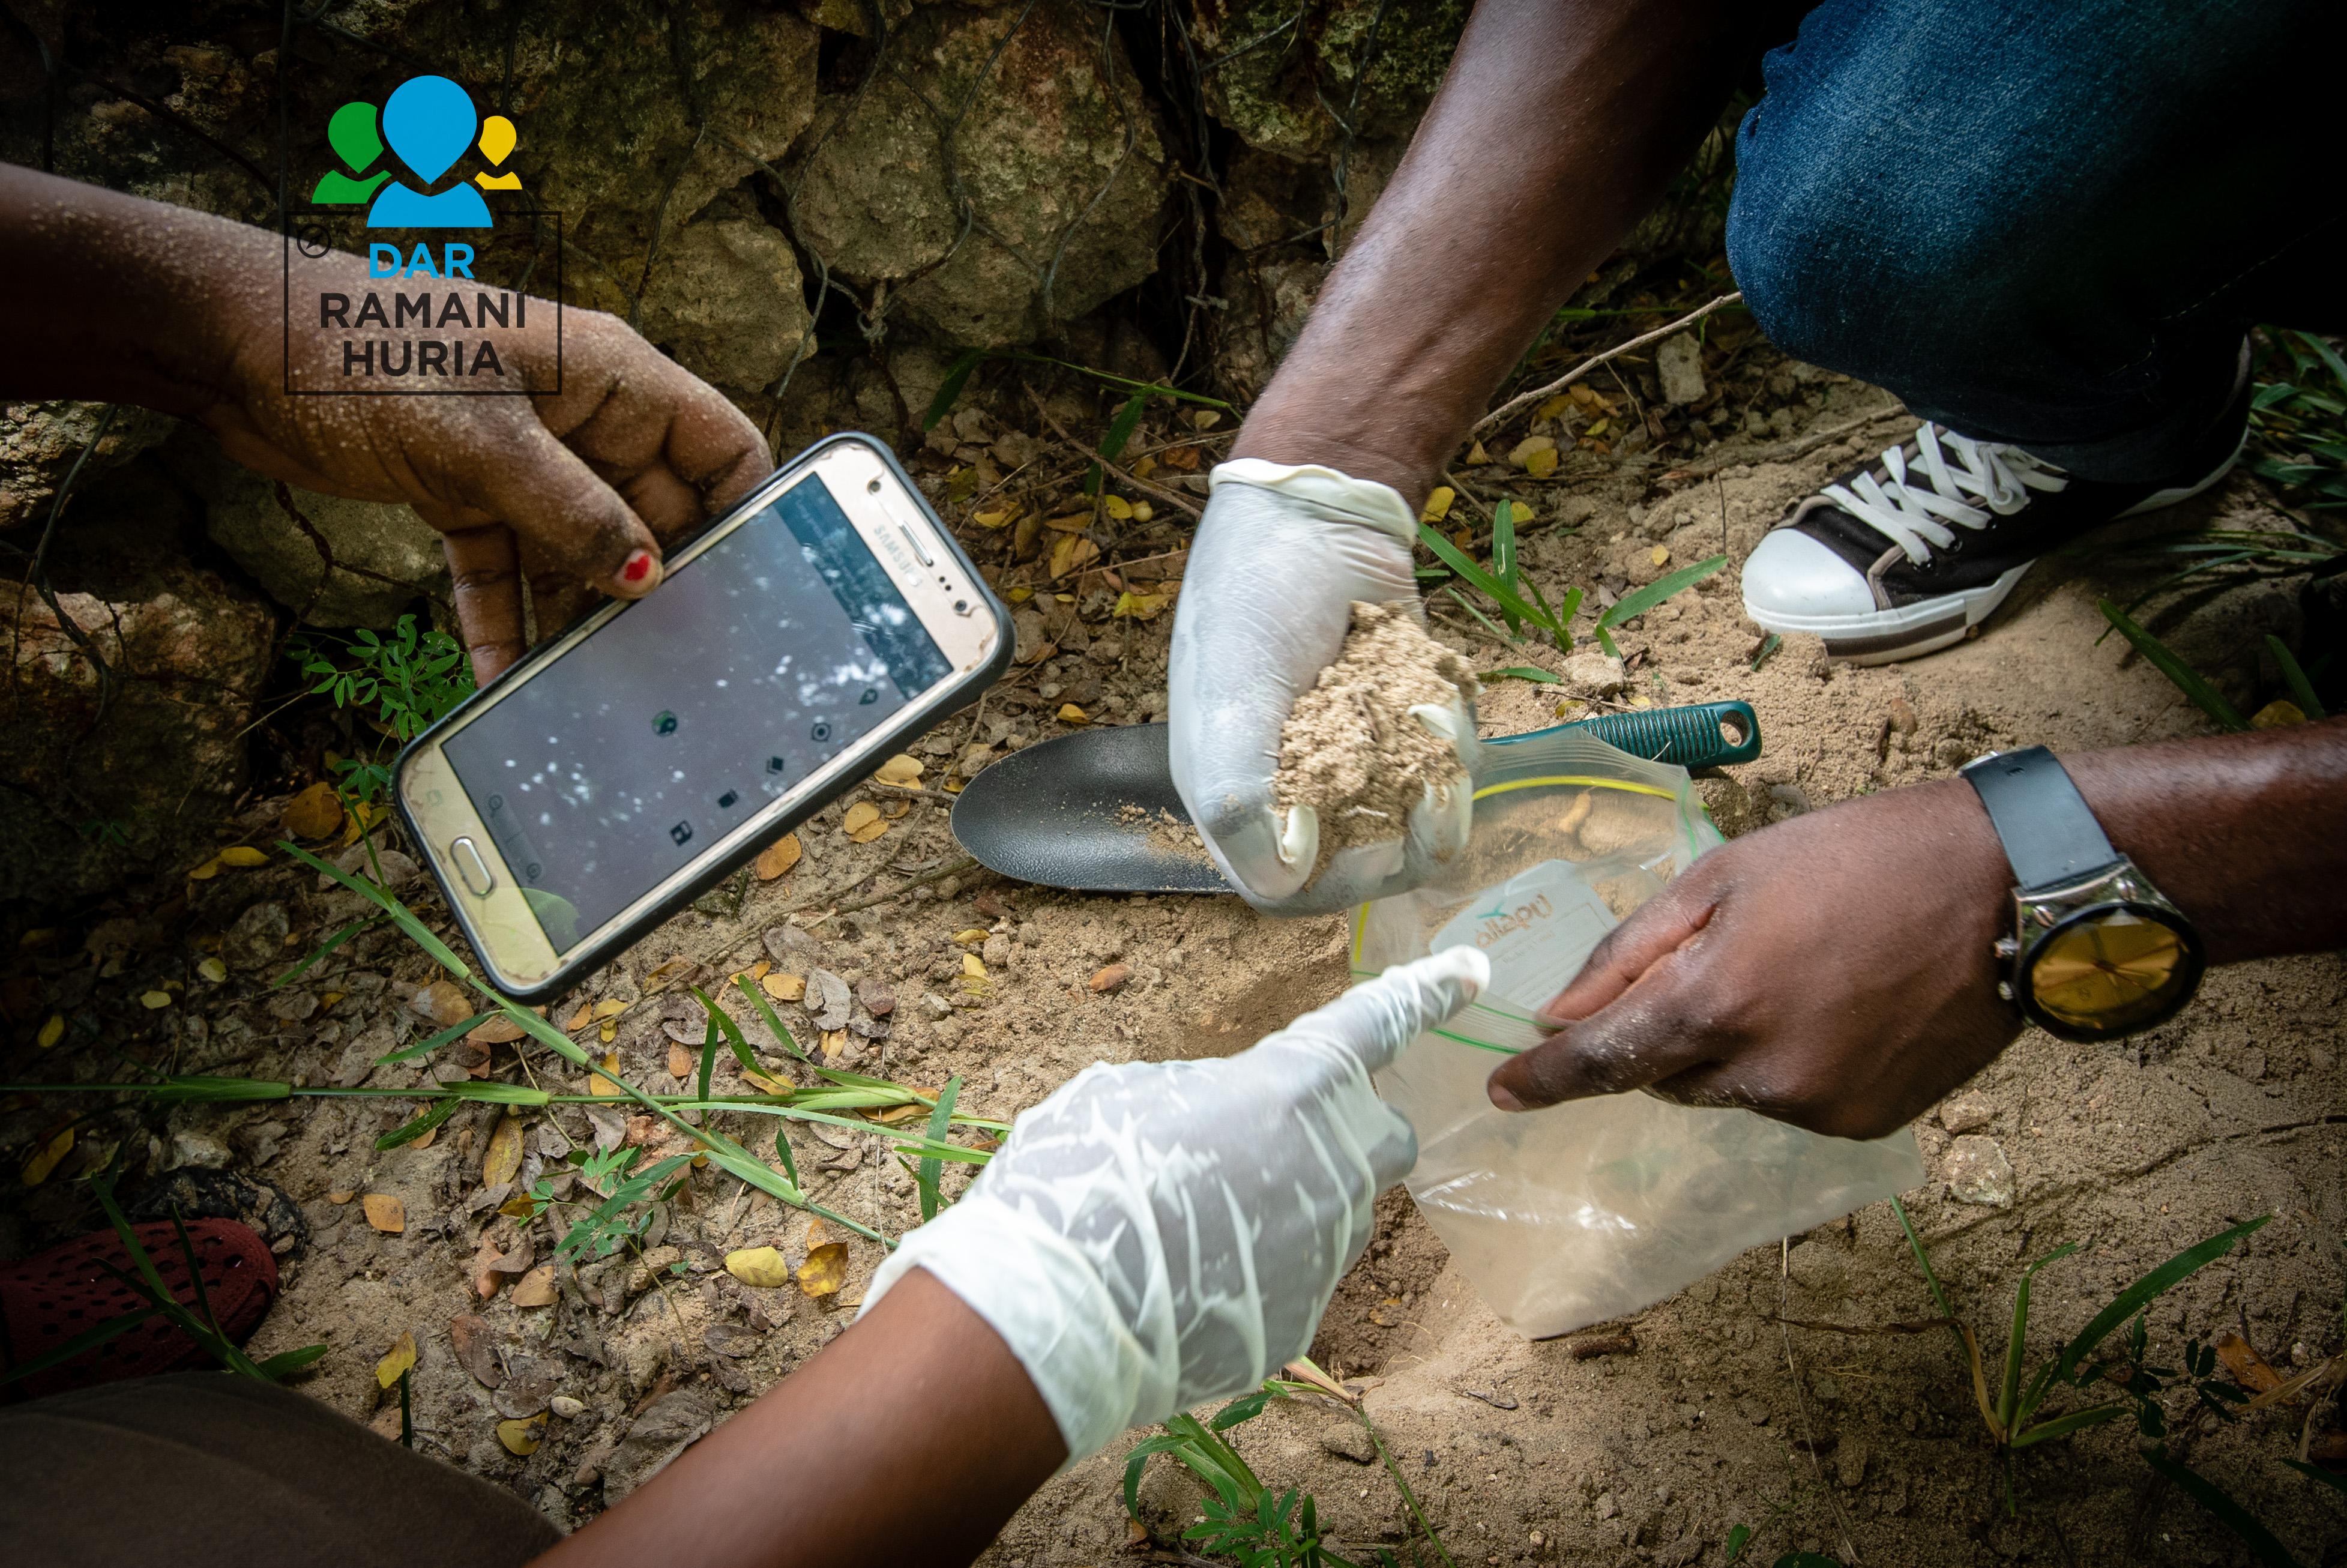
\includegraphics[width=\textwidth]{Cover_photo_with_logo.jpg}
\end{center}
\bigskip
\begin{center}
  \huge \color{RHblue} \textbf {RAMANI HURIA}

\textbf{INTERIM REPORT 4}
\end{center}
\bigskip
\vbox{
  \centering
  Prepared for:
  \vcenteredhbox{
\includegraphics[width=2cm]{UK-aid_logo.png}}
  and { }
  \vcenteredhbox{
\includegraphics[width=7cm]{World_Bank_Group_logo.png}}
  \
  
  by:
  \vcenteredhbox{
\includegraphics[width=4cm]{HOT_logo_with_text.png}}
  % \maketitle
  
}
\medskip
\begin{center}
  Humanitarian OpenStreetMap
  \
  
  15 April, 2019
\end{center}
\bigskip
\bigskip
\bigskip
\begin{center}
\color{RHblue}\rule{\textwidth}{0.6cm}
\end{center}

\newpage
\color{RHgrey}

\begin{center}
{
\includegraphics[width=5cm]{Dar_Ramani_Huria_logo.png}}
\end{center}

This report was prepared by William Evans, Innocent Maholi, Ivan Buendia Gayton, and \textcolor{red}{OTHER PEOPLE} from the Humanitarian OpenStreetMap Team in Tanzania.

\medskip

Layout and graphic design by Ivan Buendia Gayton based on the Ramani Huria design guideline by Darragh Amelia Coward, using the the \LaTeX { } typesetting system.

\medskip

Guidance and input on the project came from Edward Anderson, Caroline Gevaert, Roza Vasileva, and Msilikale Msilanga at the World Bank.

\medskip

Unless otherwise noted, photos by the Ramani Huria team.
5
 Maps were prepared by the Ramani Huria team using QGIS.

\bigskip\bigskip

\textcolor{red}{LOTS OF LOGOS}

\newpage

\tableofcontents

\newpage
\section{Executive Summary}
\label{executivesummary}
\begin{multicols}{2}
With the support of the World Bank in Tanzania, the Ramani Huria (RH) team has been collecting data for urban resilience with a particular emphasis on flooding since 2015. As the program nears its end in September of 2019, the RH team is now primarily working to curate, organize, document, and publish the data, tools and knowledge that have been created. 

We are working to transfer knowledge and hand over to Tanzania Resilience Academy, the successor project to Ramani Huria. 

Together with the coalescing Resilience Academy team, we are working to disseminate the knowledge and data to as many users---particularly those who are likely to have impact improving resilience---as possible. 

%\color{red}
Lorem ipsum dolor sit amet, consectetur adipiscing elit. Nullam sed cursus erat. Nulla et hendrerit leo. Integer ultrices volutpat mattis. In diam leo, gravida eget hendrerit non, mattis vitae enim. Vivamus malesuada varius ipsum sed venenatis. In hac habitasse platea dictumst. Aenean eget felis vel quam vehicula semper. Aenean eget luctus diam, sit amet rutrum lacus. Nulla id odio rhoncus, vestibulum lorem rutrum, faucibus felis. Aliquam erat volutpat. Donec feugiat dolor eros, a lobortis sapien vehicula ac. Quisque facilisis turpis ullamcorper magna placerat, non pulvinar tellus consectetur. Proin sit amet est malesuada, rutrum ante vitae, efficitur purus. Ut condimentum, ante id pretium fringilla, nulla leo congue augue, nec mattis erat dui tristique nunc.

Phasellus congue semper nibh nec pretium. In accumsan orci justo, egestas tincidunt neque gravida et. Nulla commodo dui efficitur, pharetra metus et, condimentum neque. Integer ac pretium enim, et congue turpis. Duis nec ex nulla. Maecenas ultricies lacus risus. Vivamus feugiat dignissim tellus, posuere eleifend lorem elementum eget. Etiam posuere odio quis nunc tincidunt gravida. Etiam lobortis augue non arcu pharetra, ut ultrices ante viverra. Maecenas ac porttitor nisl. Donec cursus libero sit amet est aliquet tristique.

Sed maximus neque magna, a consectetur ligula convallis eget. In euismod mauris eu libero condimentum, eu mattis ligula congue. Vestibulum ut nulla ut ipsum efficitur finibus. Donec viverra leo at arcu laoreet, et rhoncus nulla interdum. Morbi maximus tempor tempus. Integer vitae sodales ante. Quisque malesuada metus libero, vitae scelerisque augue iaculis vitae. Curabitur cursus nulla sollicitudin magna luctus tincidunt.

Vestibulum tempor, ligula in consectetur commodo, nisl lorem suscipit dolor, et semper quam lacus vel quam. Suspendisse potenti. Sed at pharetra odio, non porttitor tortor. Sed at massa neque. Vivamus eleifend dolor nec lacus imperdiet, et tristique augue dignissim. Donec convallis volutpat mauris, eu varius nunc tincidunt at. Integer faucibus sodales odio vel lobortis. Sed egestas magna ac varius hendrerit. Phasellus ornare lacinia libero nec fringilla. Pellentesque eu tortor consequat eros fringilla commodo condimentum sit amet arcu. Aliquam auctor ipsum ligula, vel tempor neque condimentum sodales. Fusce libero ipsum, maximus eget luctus et, viverra eget enim. Nunc sit amet nibh in nibh vulputate rutrum sit amet a metus. Nulla vitae ex sit amet urna bibendum consequat. Suspendisse malesuada volutpat magna cursus consectetur.

Nullam dignissim turpis a nulla finibus vestibulum. Aenean laoreet, turpis tempus ultrices tempus, lectus nunc tincidunt purus, quis ultricies erat lacus id quam. In velit mi, convallis quis lorem eu, semper pretium nulla. Aliquam maximus vitae mi et tempor. Morbi tincidunt tellus ac rhoncus congue. Pellentesque id risus et ex imperdiet ultrices vitae ut augue. Sed tincidunt est mauris, faucibus egestas lorem mattis sed. Nunc scelerisque rutrum dignissim. Donec laoreet maximus nunc, vitae tempor sapien euismod at. Donec posuere vehicula sapien, ac feugiat sapien ultrices vel. Integer et erat ipsum. Fusce eu nunc at neque tempus ullamcorper sit amet non purus. Praesent cursus felis nec ipsum maximus, eget mattis orci gravida. Cras est tortor, tincidunt eget augue eget, sollicitudin lacinia elit.

Nam vitae lectus ut nibh viverra auctor eu et turpis. Aenean convallis enim odio. Cras vestibulum mi eget posuere vehicula. Duis justo diam, dapibus nec tristique non, condimentum a odio. Fusce bibendum, magna et condimentum auctor, sapien magna eleifend dui, ac fermentum turpis felis quis sapien. Nam sodales sem ac nisl blandit feugiat. Vestibulum ultricies, quam sed placerat malesuada, leo turpis hendrerit est, at pretium odio massa sit amet orci. Pellentesque dignissim ex at ante tempus rutrum. Donec elementum pulvinar tempus. Nulla dignissim cursus turpis eget finibus. Pellentesque sed lorem vel enim tempor rutrum. Suspendisse massa lectus, dapibus gravida consequat at, sagittis eu diam. Donec maximus ipsum at aliquam feugiat. Proin bibendum velit nisi, vitae ultricies mauris molestie nec. Aliquam erat volutpat.

In et tincidunt ex. Donec eget ultricies leo. Mauris cursus egestas lectus, a commodo purus euismod in. Nam ac vestibulum dolor, non fringilla nibh. In eu arcu et libero elementum faucibus. Sed libero leo, dapibus non rutrum eget, volutpat quis nisi. In ligula velit, consequat nec consectetur at, vestibulum ut sapien. Lorem ipsum dolor sit amet, consectetur adipiscing elit. In interdum, nunc at venenatis aliquam, sapien ante egestas lorem, in ultrices nibh erat non erat. Pellentesque ultrices quis risus eget pulvinar. Nunc non neque eleifend, auctor neque in, cursus nunc. Maecenas purus sapien, viverra varius enim quis, dapibus suscipit diam.

Praesent et massa vulputate, viverra enim vel, mattis metus. Praesent sodales nunc ut vehicula hendrerit. Cras a sapien vel turpis tempus rutrum a tincidunt urna. Vestibulum volutpat, nisi vel mollis luctus, justo orci hendrerit sapien, at tincidunt metus sapien in ante. Nullam et scelerisque dui. Cras consequat dolor mi, a euismod nibh auctor ut. Ut ipsum dui, finibus ut imperdiet sit amet, volutpat in erat. Donec molestie lacus quis tortor mollis scelerisque. Lorem ipsum dolor sit amet, consectetur adipiscing elit. Aenean eros sapien, molestie id aliquet ac, laoreet quis risus. Cras malesuada metus sit amet laoreet egestas. Pellentesque ullamcorper arcu vel accumsan mattis. Nullam et auctor est. Proin nisi leo, gravida sit amet lectus ut, posuere lacinia ligula. Suspendisse dictum mollis massa et posuere. Ut mollis urna in velit sodales, nec sodales augue scelerisque.

\end{multicols}

%\includegraphics[width=0.8\textwidth]{sample_locations.jpg}

\newpage
\section{Introduction}
\label{Introduction}

This report will tell you about stuff

\begin{itemize}
  \item Like this
  \item And this
\end{itemize}

We also would like to point out a link to  \href{https://ramanihuria.org}{a website}\footnote{\url{http://ramanihuria.org}\color{RHgrey} { }because it's really, really interesting. You should click on that link.}. Did you notice that there was a footnote there? If you look at the footnote it contains the full URL of the link, so that people reading the document on paper can see what it links to? Cool, huh? The rest of the text on this page will be in two columns, just because we can do that with the \LaTeX{} \textbf{\textit{multicols}} plugin. By the way, I can highlight code with a color box like \textbf{\colorbox{code}{this.}}

\begin{multicols}{2}
\color{red}
Lorem ipsum dolor sit amet, consectetur adipiscing elit. Nullam sed cursus erat. Nulla et hendrerit leo. Integer ultrices volutpat mattis. In diam leo, gravida eget hendrerit non, mattis vitae enim. Vivamus malesuada varius ipsum sed venenatis. In hac habitasse platea dictumst. Aenean eget felis vel quam vehicula semper. Aenean eget luctus diam, sit amet rutrum lacus. Nulla id odio rhoncus, vestibulum lorem rutrum, faucibus felis. Aliquam erat volutpat. Donec feugiat dolor eros, a lobortis sapien vehicula ac. Quisque facilisis turpis ullamcorper magna placerat, non pulvinar tellus consectetur. Proin sit amet est malesuada, rutrum ante vitae, efficitur purus. Ut condimentum, ante id pretium fringilla, nulla leo congue augue, nec mattis erat dui tristique nunc.

Vestibulum malesuada est mauris, in dictum augue gravida ac. Sed nec augue scelerisque, tincidunt ipsum vel, auctor nunc. Nam feugiat lorem et tellus scelerisque, sed feugiat sapien sagittis. Interdum et malesuada fames ac ante ipsum primis in faucibus. Suspendisse orci augue, aliquam ac tortor in, sodales efficitur dui. Duis ultricies bibendum libero, vitae vulputate dolor blandit sit amet. Suspendisse cursus posuere diam, vitae ornare purus elementum sed. Cras vitae felis cursus, pellentesque quam eget, consequat risus. Quisque vehicula porttitor turpis id tincidunt. Aliquam erat volutpat. Morbi et felis augue. Donec aliquam mi sit amet turpis rutrum imperdiet. Cras odio nisi, auctor ut vehicula aliquet, posuere cursus arcu. Nam dui urna, semper ut sem sit amet, mattis sodales mauris. Nulla est tellus, maximus nec porta non, vestibulum id quam.

Phasellus congue semper nibh nec pretium. In accumsan orci justo, egestas tincidunt neque gravida et. Nulla commodo dui efficitur, pharetra metus et, condimentum neque. Integer ac pretium enim, et congue turpis. Duis nec ex nulla. Maecenas ultricies lacus risus. Vivamus feugiat dignissim tellus, posuere eleifend lorem elementum eget. Etiam posuere odio quis nunc tincidunt gravida. 

\end{multicols}

\newpage
\section{Monthly Activity Summary}

The graphic below shows all the stuff we did in each month! Wow!

\bigskip

\begin{itemize}
    \item October 2018
Drainage Mapping
Hyper-local administrative boundary mapping
Soil sampling
Tabata Trash Mapping
    \item November 2018
Hyper-local administrative boundary mapping
Soil sampling
Tabata Trash Mapping
    \item December 2018
Hyper-local administrative boundary mapping
Soil sampling
Tabata Trash Mapping
Asset and Threat Mapping
Data publication on GeoNode with Uhurulabs
    \item January 2019
Drainage mapping
Tabata Trash Mapping
Asset and Threat Mapping
    \item February 2019
Soil sampling
Tabata Trash Mapping
Drainage Mapping
Asset and Threat Maps Production
Data Quality Assurance
Data publication on GeoNode with Uhurulabs
\end{itemize}

\section{Team Composition and Assignments}
Hi there!

\section{Data Quality}
This is the data quality process. 

We do the following steps


\section{Datasets}
Here are some descriptions of datasets!

\newpage
\subsection{Community Assets and Threats}

\begin{multicols}{2}
Community asset and threat inventory is a project that falls under pillar one in Tanzania Urban Resilience Programme (TURP) focusing on risk identification. TURP aims at mitigating risks through coordinated and strategic actions led by the Government of Tanzania with support from the World Bank and the UK Department for International Development. This programme works in risk identification, risk reduction, and emergency preparedness.
The project begun from July-December 2018  conducted through local engagement  in order to access well-informed local knowledge. The aim is to understand key assets (resources or things that the community feels are important in their subward) and potential threats---in this inventory this was based on flood hazards. Community assets referred here are schools, hospitals, religious institutions, businesses, etc. and threats mean assets usually flooded or are at risk of flooding. This information can only be provided by the community itself since they understand their neighbourhoods better. The inventory covered  243 subwards in 49 wards of Dar es Salaam. 
\end{multicols}

\subsubsection{Spatial Extent}

\begin{figure}[h]
  \color{RHgreen}\caption{49 Wards covered during the community asset and threat mapping inventory}
  \centering
  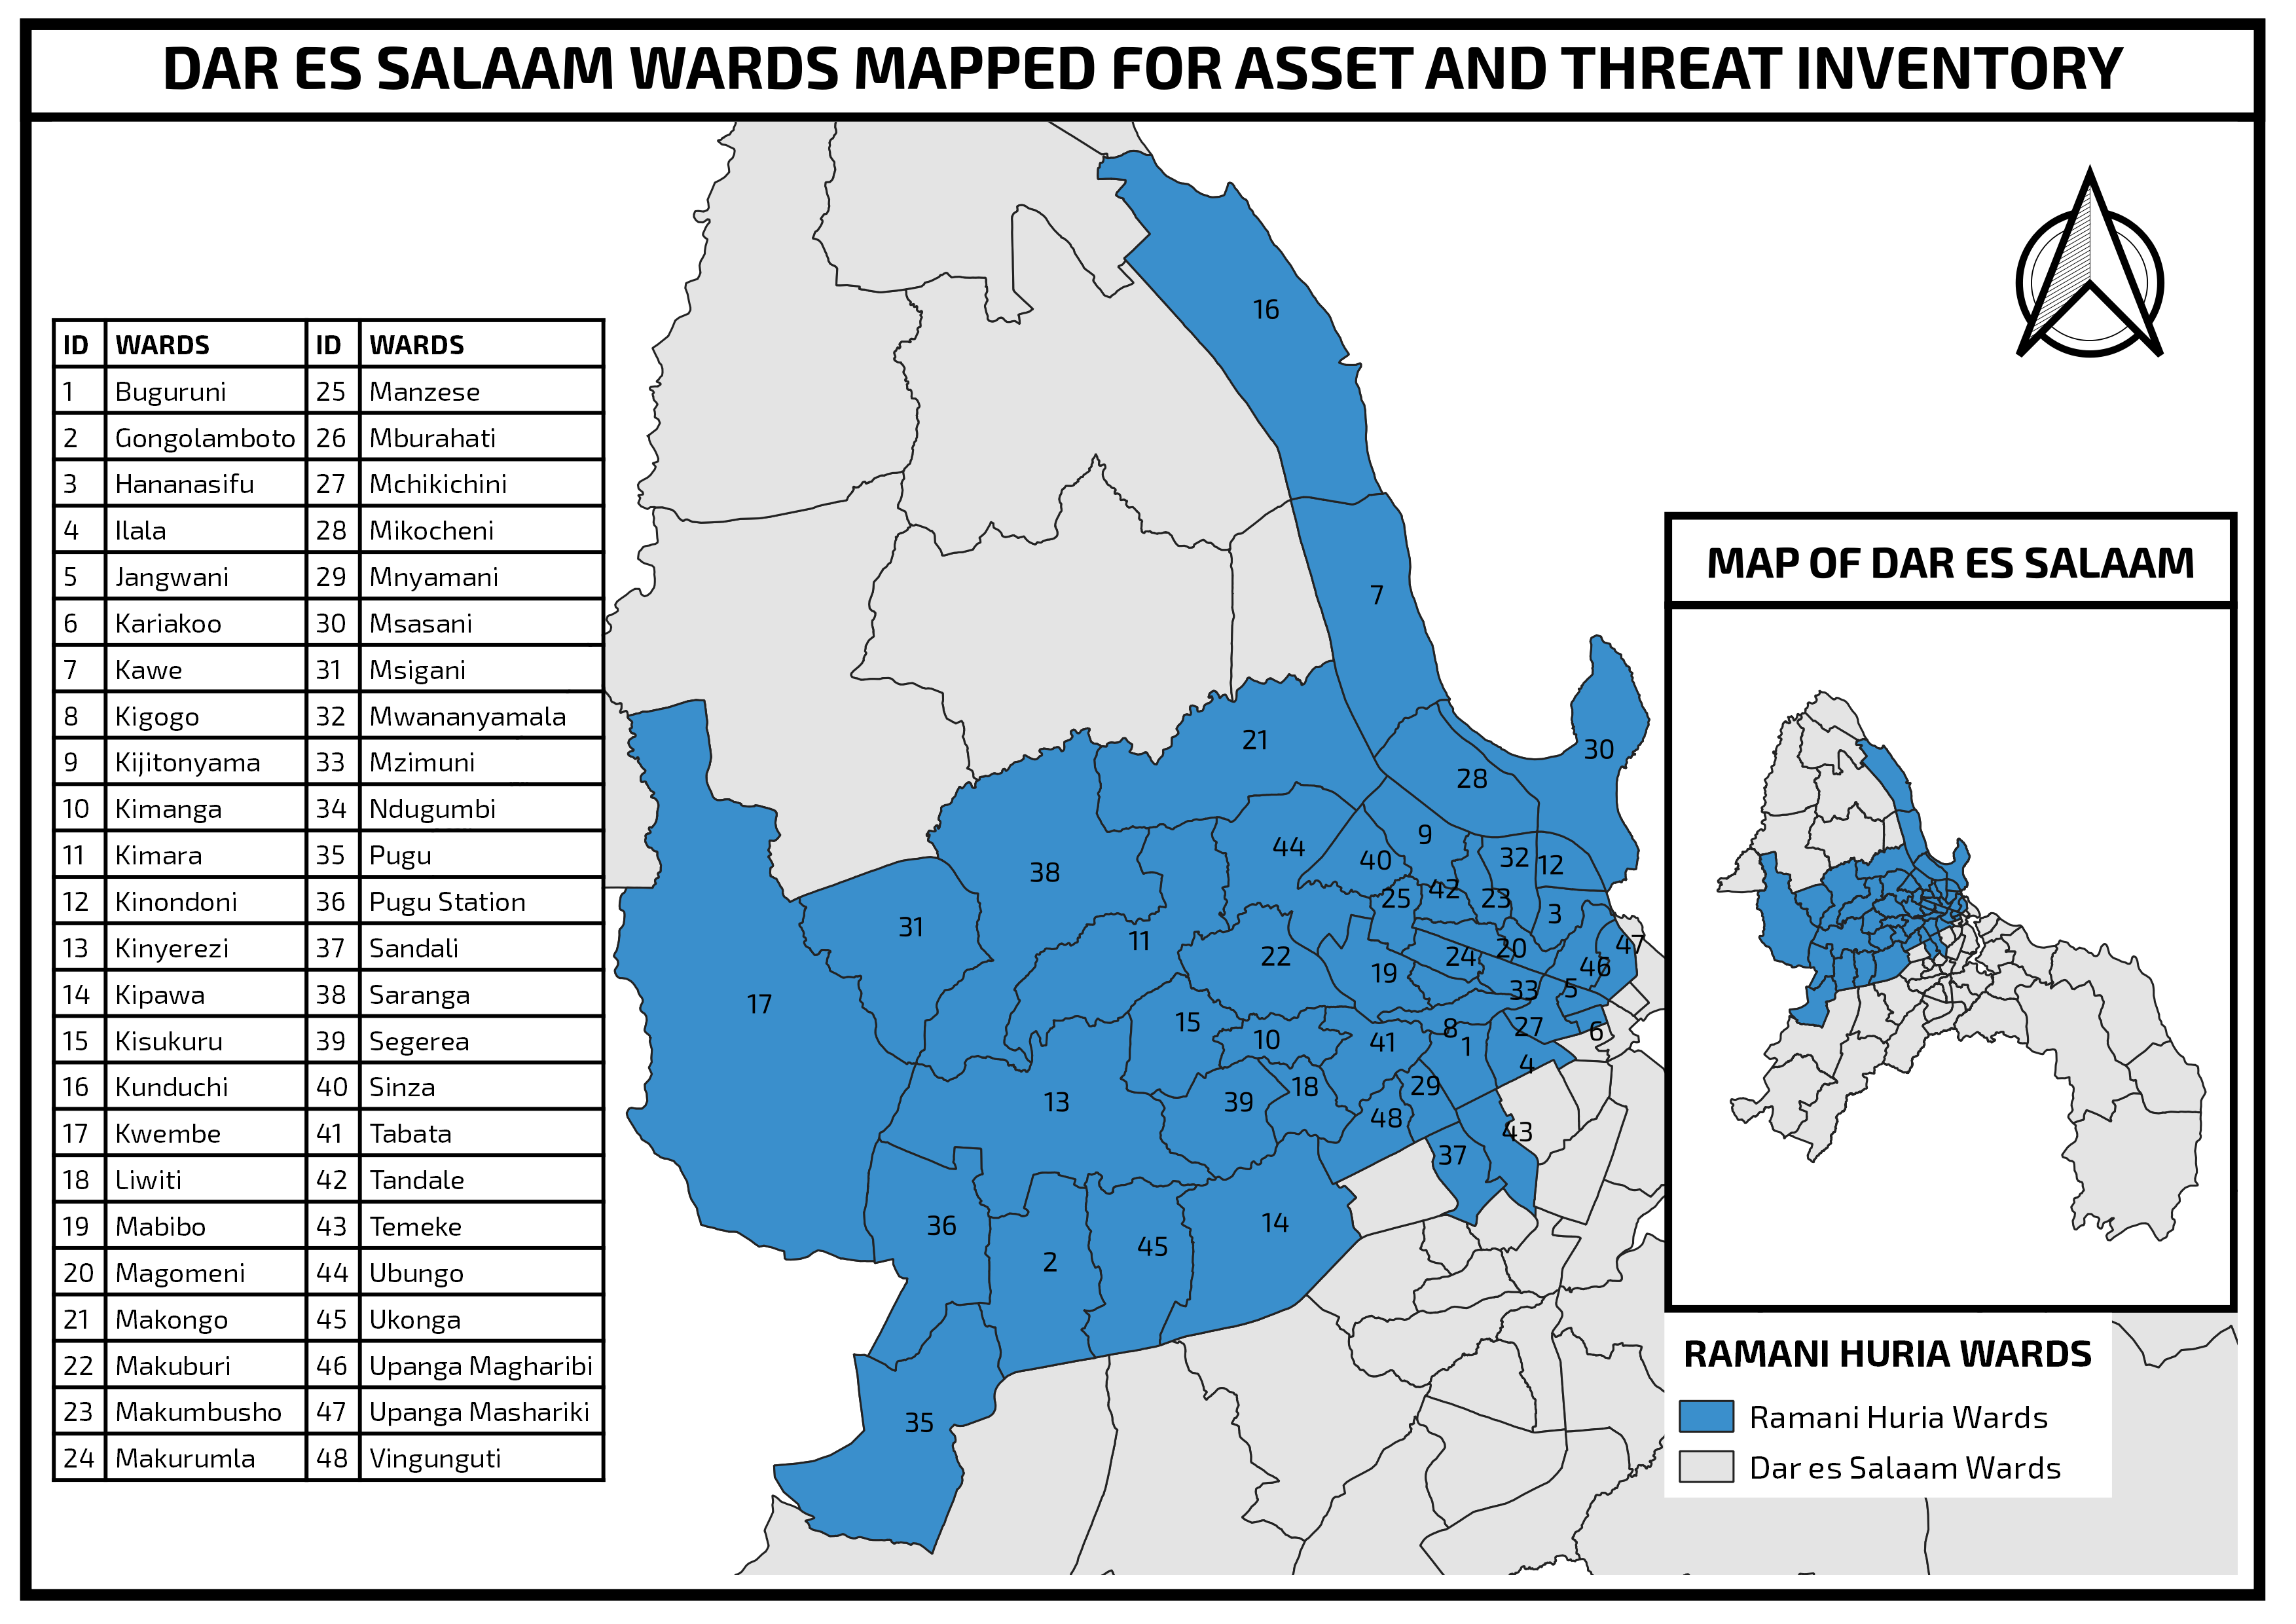
\includegraphics[width=0.8\textwidth]{images/asset_and_threat_wards.png}
\end{figure}

\subsubsection{Data Collection Methodology}

We met with people and asked them questions.

Sometimes they answered sensibly. Sometimes not. Sometimes we wrote down the answers. Sometimes not.

\subsubsection{Data Model}

A total of 5020 asset points were collected during the project. These include:
\begin{itemize}
    \item Assets at risk but not important---28 
    \item Evacuation centers---42
    \item Important assets and at risk---857
    \item Important assets but not at risk---4093
    \item Roads and road names, and
    \item Landmarks
\end{itemize}

\subsubsection{Timeline}
06/08/2018 to January, 2019

\subsubsection{Quality Assurance}
Excel, JOSM for buildings and assets and QGIS for roads

\subsubsection{Data Visualization}

\subsubsection{Use Case}
March, 2019 community flood response, creating resilience plans, mitigation measures through community mapping and impact assessment.

\subsubsection{Data Gap}
Out of 49 wards, historical flood extent was conducted in only 11 wards. There is a need of conducting flood extent in the remaining wards to create a better understanding of flooding.

\subsubsection{Lessons Learned}
Community members should “never” be neglected during data collection in their neighbourhoods. They understand the extent very well, severity and pattern than anyone else because of the experience they have and how much the scenario affects them.

\newpage
\subsection{Flood Extents}

Historical flood extent covered areas that are mostly affected by floods during rainy seasons. Households surveys were conducted to capture details in  subwards of the respective wards across the Msimbazi River rivers and streams that outflow to the main river.

\medskip

The information captured aimed to know whether the respondent had been affected by floods in the previous years, the flood depth and flood occurrence years---historical flood events. Individuals were asked to reflect on historical flood extents; therefore there is inherent subjectivity in their memories

\subsubsection{Spatial Extent}
\begin{figure}[h]
  \color{RHgreen}\caption{Map showing the flood extent progress in Dar es Salaam}
  \centering
  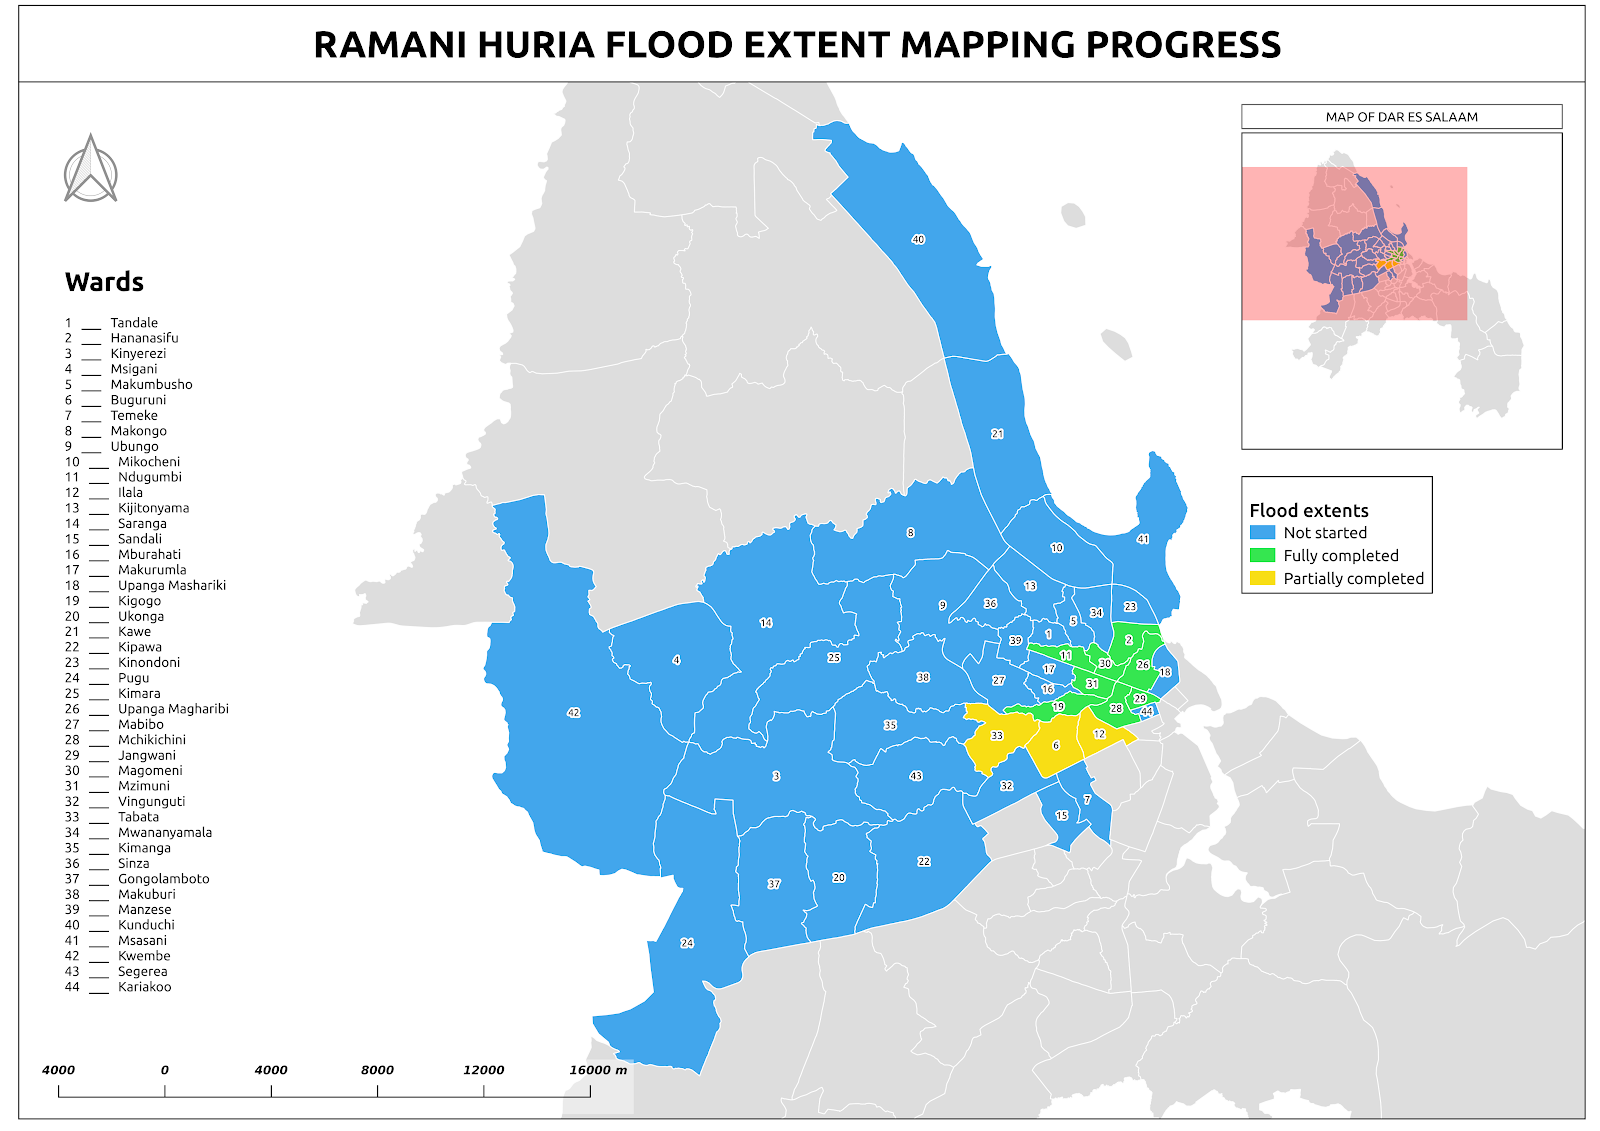
\includegraphics[width=1\textwidth]{images/RH_Flood_Extent_Progress.png}
\end{figure}

\subsubsection{Data Collection Methodology}

We met with people and asked them questions.

Sometimes they answered sensibly. Sometimes not. Sometimes we wrote down the answers. Sometimes not.

\subsubsection{Data Model}

\subsubsection{Timeline}
24/08/2017 to 12/04/2018

\subsubsection{Quality Assurance}
QGIS, Excel

\bigskip
People said all kinds of crazy crap. We checked on it.

We ourselves often wrote down ridiculous things. We checked them.

Our tracing and field mapping was sometimes awful. We looked for mistakes and corrected them.

\subsubsection{Statistics}
11 out of 44 prioritized Ramani Huria wards mapped, 30 000 household surveys

\subsubsection{Data Visualization}

\subsubsection{Use Case}

\subsubsection{Data Gap}
Individuals were asked to reflect on historical flood extents; therefore there is inherent subjectivity in their memories

\subsubsection{Lessons Learned}

\newpage
\subsection{Drainage}
Drainage data collected in the most flood prone areas across Dar es Salaam using cheap  and practical methods. This information will be used to develop a flood model which requires accurately collected specifications of drains such as depth, width, blockage (by either vegetation or material), connectivity, and diameter (typically for culverts).

\subsubsection{Spatial Extent}
\begin{figure}[h]
  \color{RHgreen}\caption{Map showing the drainage mapping progress as of March, 2019}
  \centering
  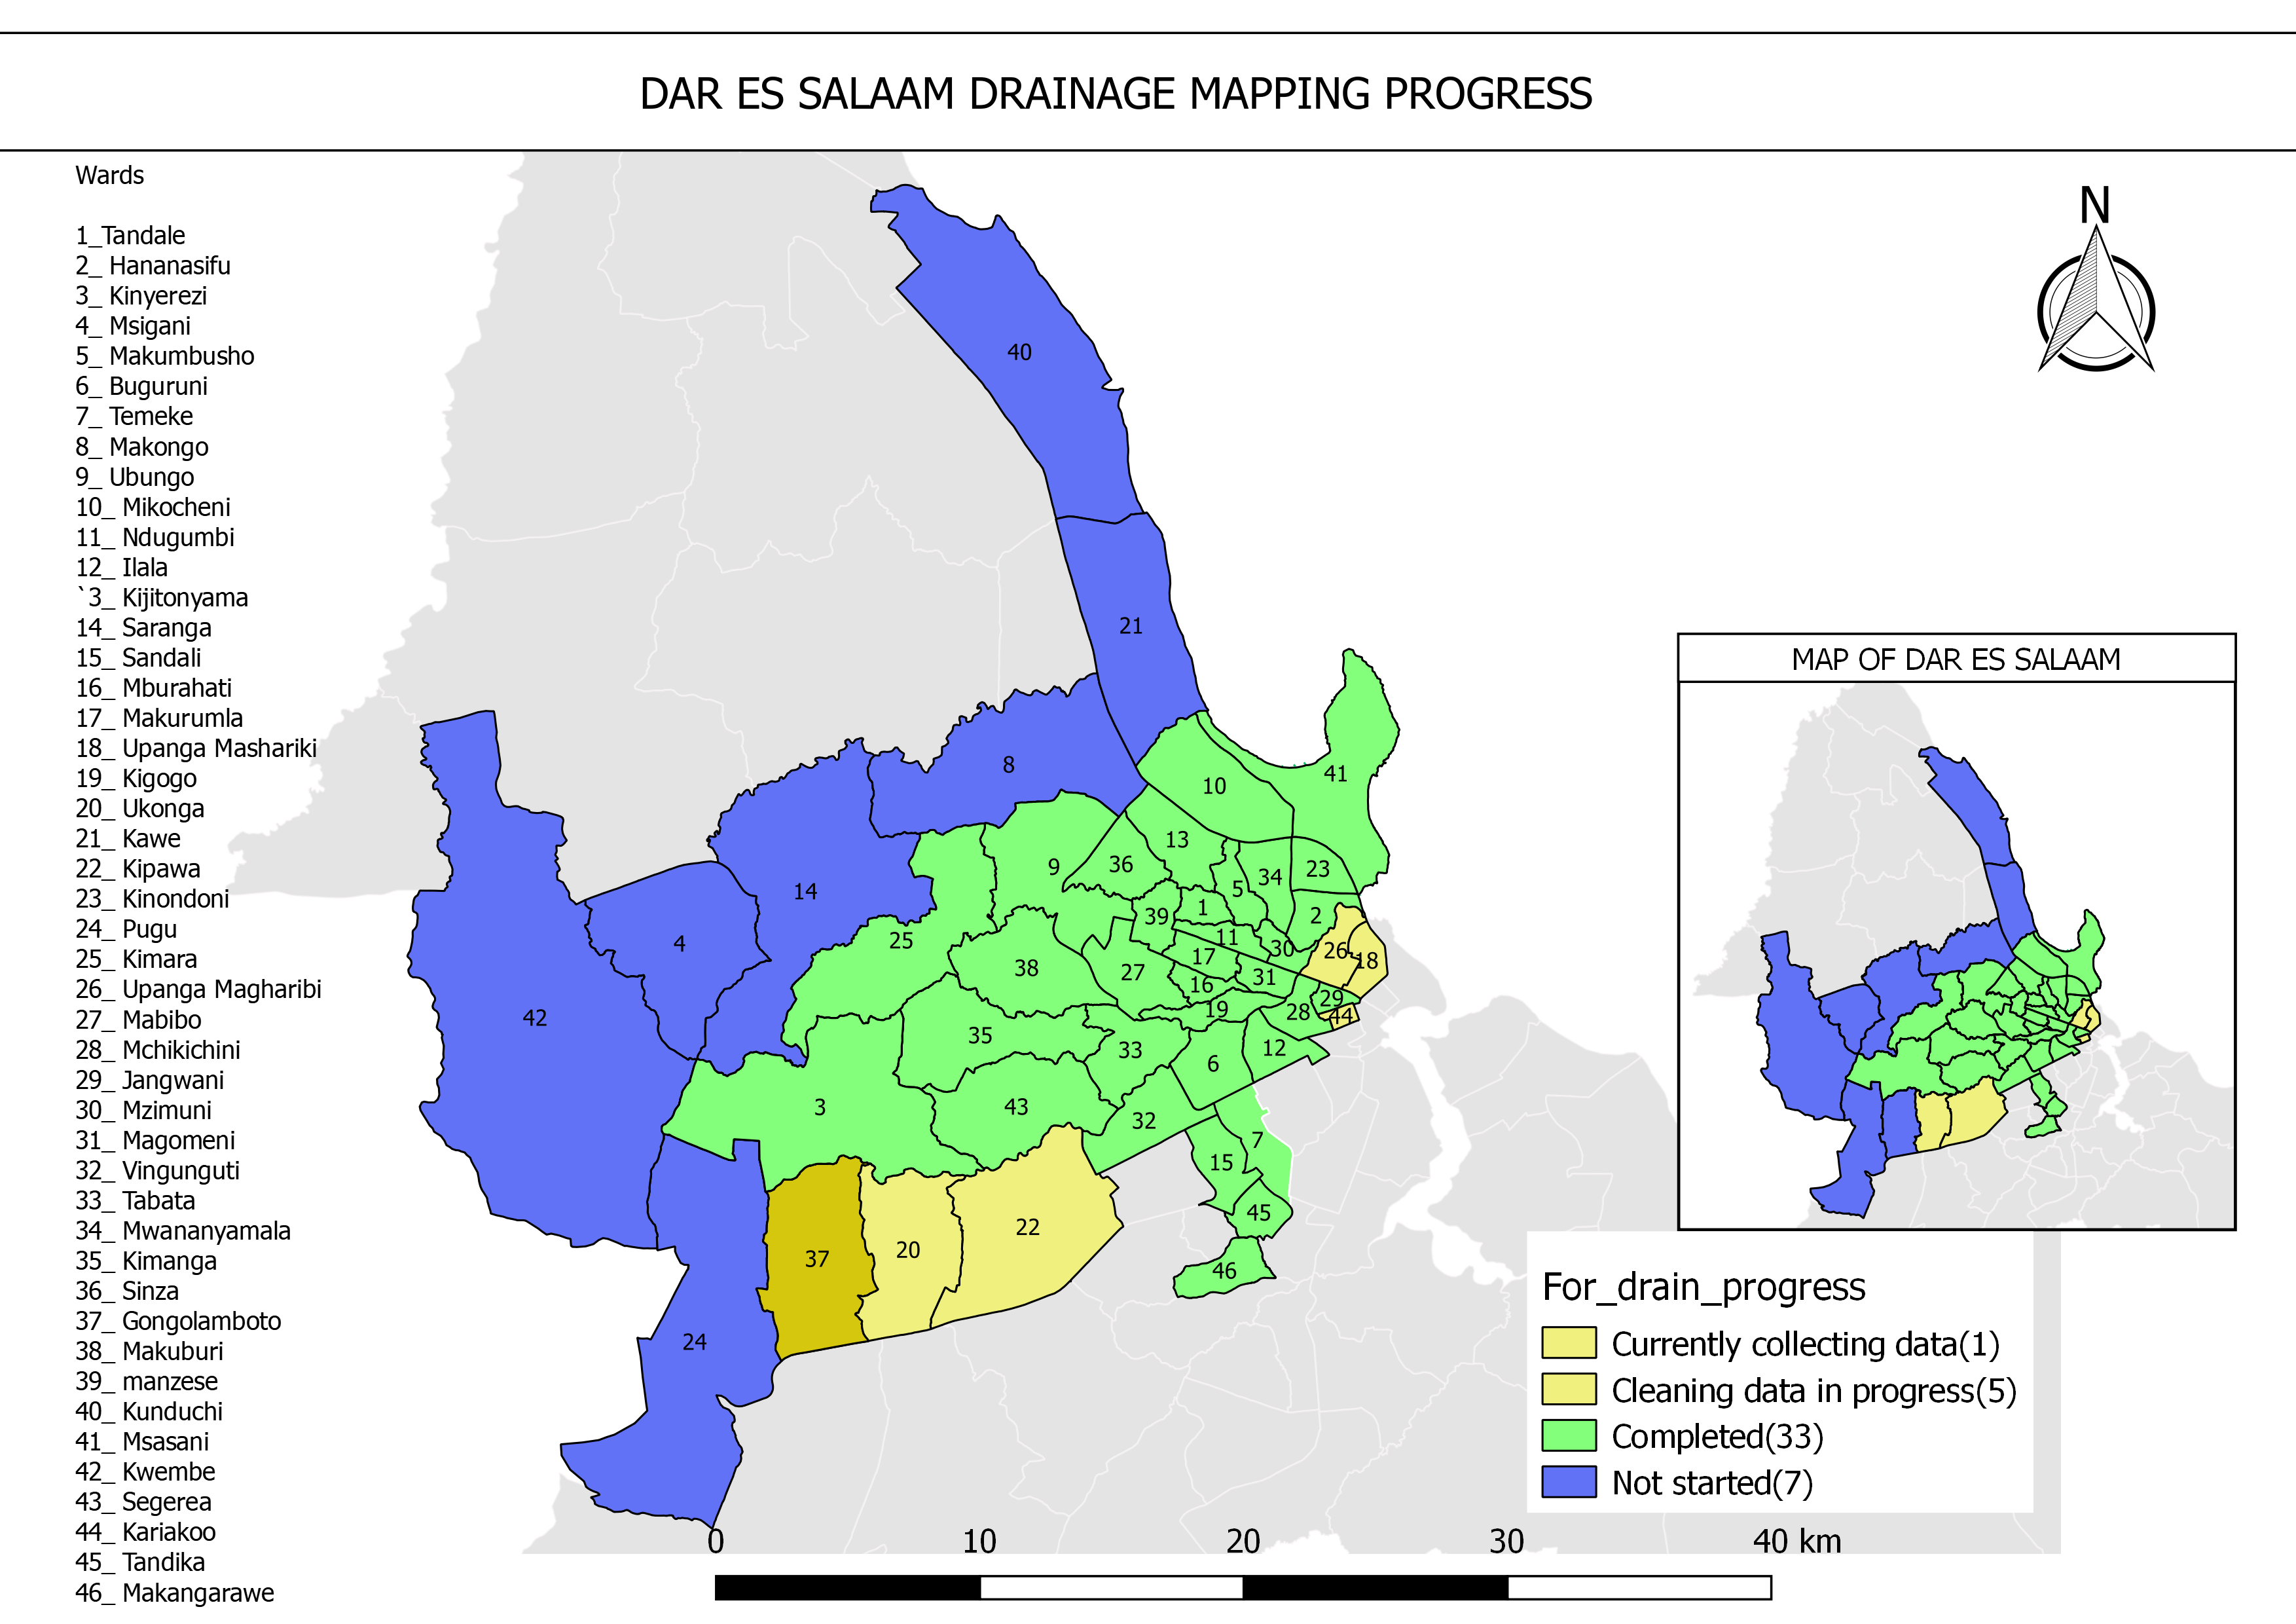
\includegraphics[width=1\textwidth]{images/Dar_drainage_mapping_progress.png}
\end{figure}

\subsubsection{Data Collection Methodology}

Drain points and segments data were traced using ODK Collect application. So far, drainage mapping has been completed in 38 wards of Dar es Salaam and 1 ward is still under cleaning process.

\subsubsection{Data Model}
\href{https://wiki.openstreetmap.org/wiki/Dar_es_Salaam/Ramani_Huria}{https://wiki.openstreetmap.org/wiki/Dar es Salaam/Ramani Huria}

\subsubsection{Timeline}
August, 2017 to Ongoing

\subsubsection{Quality Assurance}

Drainage data is cleaned using QGIS, a high resolution 2016 COWI imagery and in Hydro osm python model.

\subsubsection{Statistics}
38 out of 44 wards of Dar es Salaam Ramani Huria prioritized wards completed

\subsubsection{Data Visualization}

\subsubsection{Use Case}
Development of a flood model and early warning systems

\subsubsection{Data Gap}

\subsubsection{Lessons Learned}

\newpage
\subsection{Buildings and Infrastructure}
\begin{multicols}{2}
Re-digitization of the city to update and improve the quality of already digitized layers using COWI imagery with 10cm resolution provided by the Ministry of Lands, Housing and Human Settlements. (Previously the city was digitized using either Bing, Mapbox or Digitalglobe which have lower resolutions compared to COWI imagery. So far the team has been able to digitize 28 out of 44 Ramani Huria wards. Namely Kisutu, Temeke, Vingunguti, Upanga Mashariki, Upanga Magharibi, Jangwani, Sandali, Kivukoni, Mwananyamala, Tabata, Kigogo, Kariakoo, Gerezani, Mchikichini, Hananasifu, Sinza, Kjitonyama, Magomeni, Tandale, Buguruni, Ilala, Keko, Mbagala, Mbagala kuu, Mabibo, Mchafukoge and Mzimuni. The wards digitized have a total of 299,691 buildings. This number includes new and existing buildings altogether.
\end{multicols}

\subsubsection{Spatial Extent}

\subsubsection{Data Collection Methodology}

We traced buildings, we visited buildings, and we looked for things. We put them in OpenStreetMap.

\subsubsection{Data Model}
\href{https://wiki.openstreetmap.org/wiki/Dar_es_Salaam/Ramani_Huria}{https://wiki.openstreetmap.org/wiki/Dar es Salaam/Ramani Huria}

\subsubsection{Timeline}
24/08/2018 to 20/10/2018

\subsubsection{Quality Assurance}
JOSM

\subsubsection{Statistics}
28 wards have been re-digitized, though all 95 wards are digitized

\subsubsection{Data Visualization}

\subsubsection{Use Case}
Apart from showing how buildings are arranged, the digitized data has been used in other Ramani Huria activities such as Green WastePro and Assets and Threat Mapping.

\subsubsection{Data Gap}

\subsubsection{Lessons Learned}

\newpage
\subsection{Administrative Divisions and Landmarks}
Hyperlocal boundaries are divisions within subwards regarded as political boundaries previously referred to as ten cell divisions as they were originally comprised of ten households.
Due to the increase in population, they comprise of 30 to 200 households and are administered by local leaders (wajumbe). Wajumbe are increasingly functioning as non-partisan public servants, often the first---in most cases---point of interaction between the government and citizens.
Given the rate of urbanization in Dar es Salaam, it is very difficult to locate people and their respective addresses due to the unplanned and informal nature of these communities. Using more granular boundaries however makes it easier to locate people and provide services more precisely. 

\subsubsection{Spatial Extent}
\begin{figure}[h]
  \color{RHgreen}\caption{Map showing Ramani Huria collaboration with Data Zetu hyper-local boundaries mapping}
  \centering
  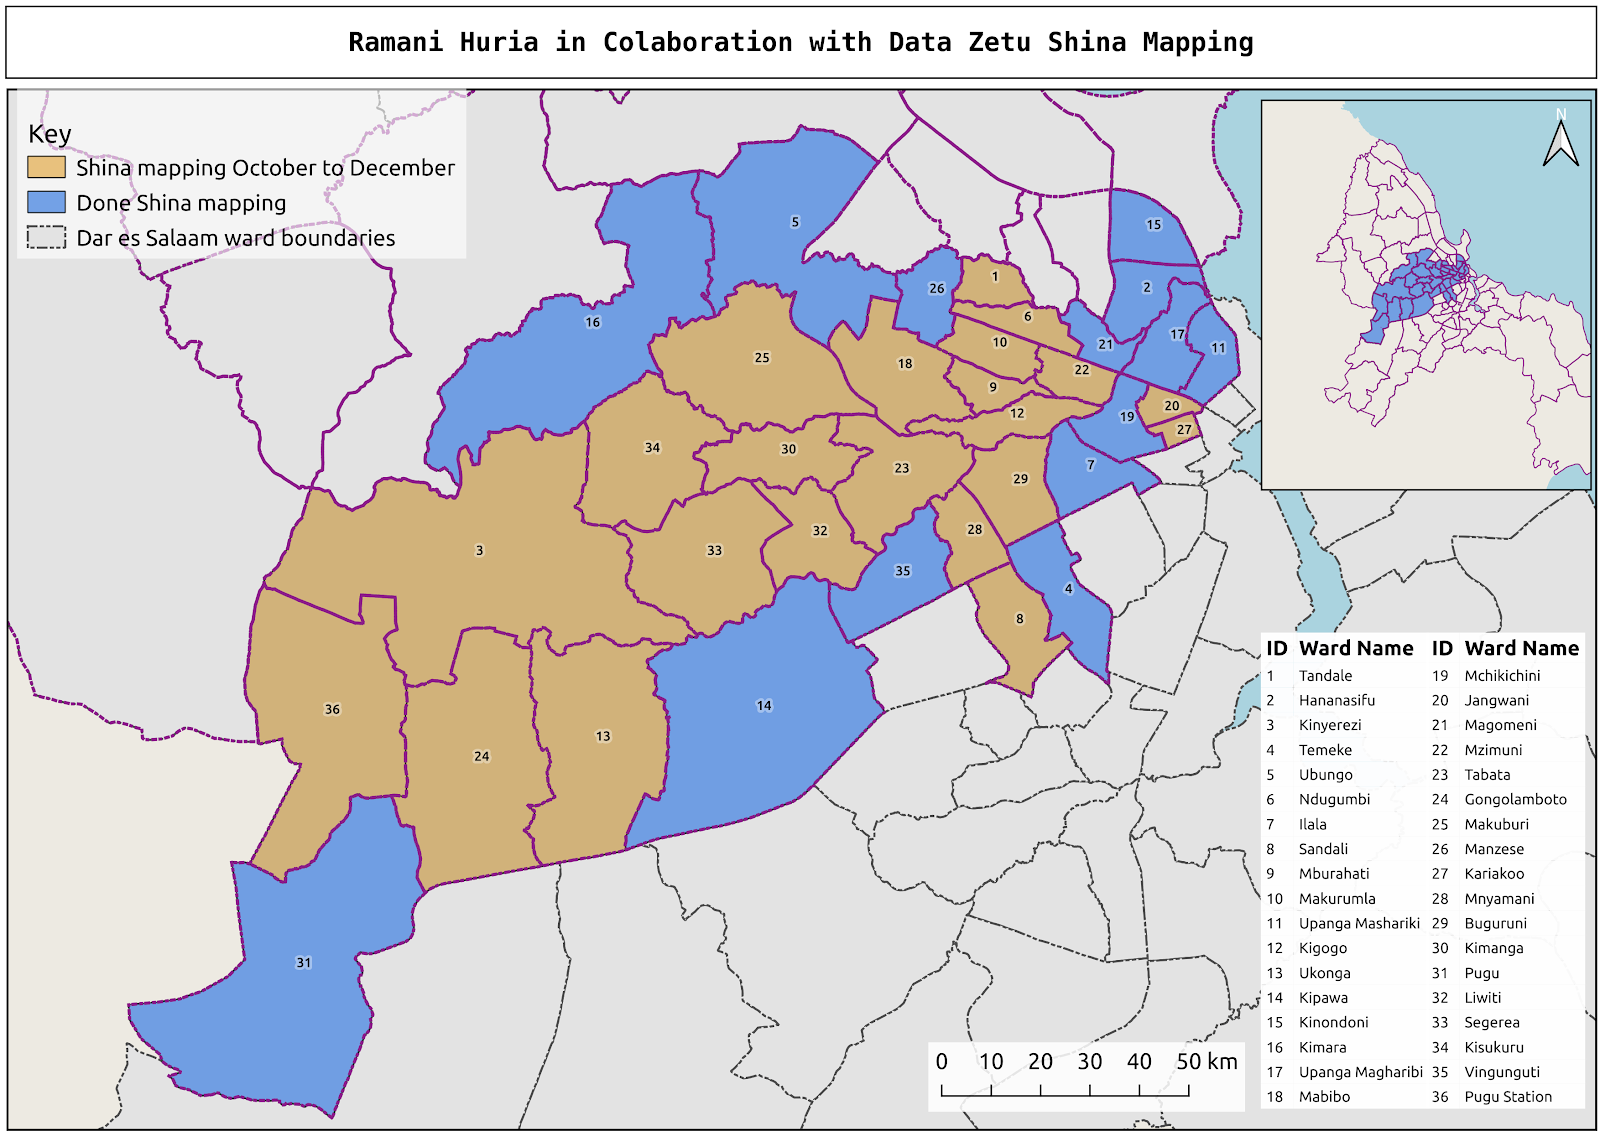
\includegraphics[width=0.8\textwidth]{images/RH_DZ_shina_boundaries.png}
\end{figure}

\subsubsection{Data Collection Methodology}

\subsubsection{Data Model}

\subsubsection{Timeline}
13/09/2018 to 24/12/2018

\subsubsection{Quality Assurance}
QGIS, Excel

\subsubsection{Statistics}
2612 hyperlocal boundaries mapped in 35 wards of Dar es Salaam

\subsubsection{Data Visualization}

\subsubsection{Use Case}
To find people’s address in Dar es Salaam, \href{https://www.hotosm.org/updates/piloting-tanzanias-first-patient-origin-tracking-system/}{Amana Hospital patient origin tracking system}\footnote{\url{https://www.hotosm.org/updates/piloting-tanzanias-first-patient-origin-tracking-system/}}

\subsubsection{Data Gap}
All hyperlocal boundaries have been cleaned and verified for map production except Mabibo subward. The team faced political misunderstandings among wajumbe as most of the hyperlocal boundaries overlapped among different political parties and made it difficult for the team to trace the boundaries.

\subsubsection{Lesson Learned}

\newpage
\subsection{Soil Sediment Sampling}

With the support of the World Bank in Tanzania, Ramani Huria and JBA Consulting partnered to develop a surface soil dataset for the greater Dar es Salaam region of Tanzania. This was intended to support a geomorphological assessment taking into account soil characteristics for erosion and flood risk studies.

\medskip

A national-level soil profile had existed for Tanzania prior to this effort, but contained only a single sample from Dar es Salaam. This was not sufficient to analyse erosion potential across the city. The JBA team in consultation with Ramani Huria decided to use a 2km grid, which resulted in 731 sampling points being pre-established throughout the city.

\subsubsection{Spatial Extent}

\subsubsection{Data Collection Methodology}

\begin{multicols}{2}
A set of data was recorded at each site using OpenDataKit’s Android application ODK Collect. The team developed a form specific to this exercise. It included a GPS point, selection from a list of the Region, District, Ward, and Subward, the ID number of the sample site (from the numbering of the 2km 
grid), a photograph before, during, and after the collection, information on accessibility, a note if the weather was wet or dry, characteristics of the site (loose or consolidated sediment, low, medium, or high vegetation cover, rural or urban setting) and a photo facing outward from the site in each cardinal direction.

Each field sampling team of two people carried the following equipment: trowel or small shovel, plastic “ziploc” bags with 1kg capacity, Android phone pre-loaded with ODK Collect, a separate maps and navigation application, maps.me, pre-loaded with the locations to be visited (the 2km grid), first aid kit, marker pens, permission letter for the sampling activity from the municipal authorities and a tape measure.

The pair of samples—top and bottom—from each site was passed through a set of progressively finer-mesh sieves, resulting in nine separate fractions. Each fraction was weighed. The resulting measurements, which represent the proportion of each sediment particle size at each site, were
recorded.

The following materials were used: a set of metal sieves, scales, hand wash station and gloves, brush, cloth, and towel for cleaning sieves, Android phone with ODK Collect and sieving survey.
\end{multicols}

\subsubsection{Data Model}

\subsubsection{Timeline}
11/10/2018 to 23/02/2019

\subsubsection{Quality Assurance}

The 643 samples were analyzed by sieving each to separate the soil by particle size and weighing the resulting fractions for analysis. The resulting dataset, a geo-referenced set of soil profiles, has been published as open data.

\bigskip

Sometimes we didn't weigh the dirt properly, or we didn't write down the correct number from the scale after we weighed the dirt. That was bad. 

We had to go get a lot more dirt. Then we had to sieve and weigh it again. That was expensive, but it worked and now we have a nice dataset.

\begin{figure}[h]
  \color{RHgreen}\caption{This is a picture we are labeling as a figure---it's really nice, no? The text of the figure is green. Green is a nice color.}
  \centering
  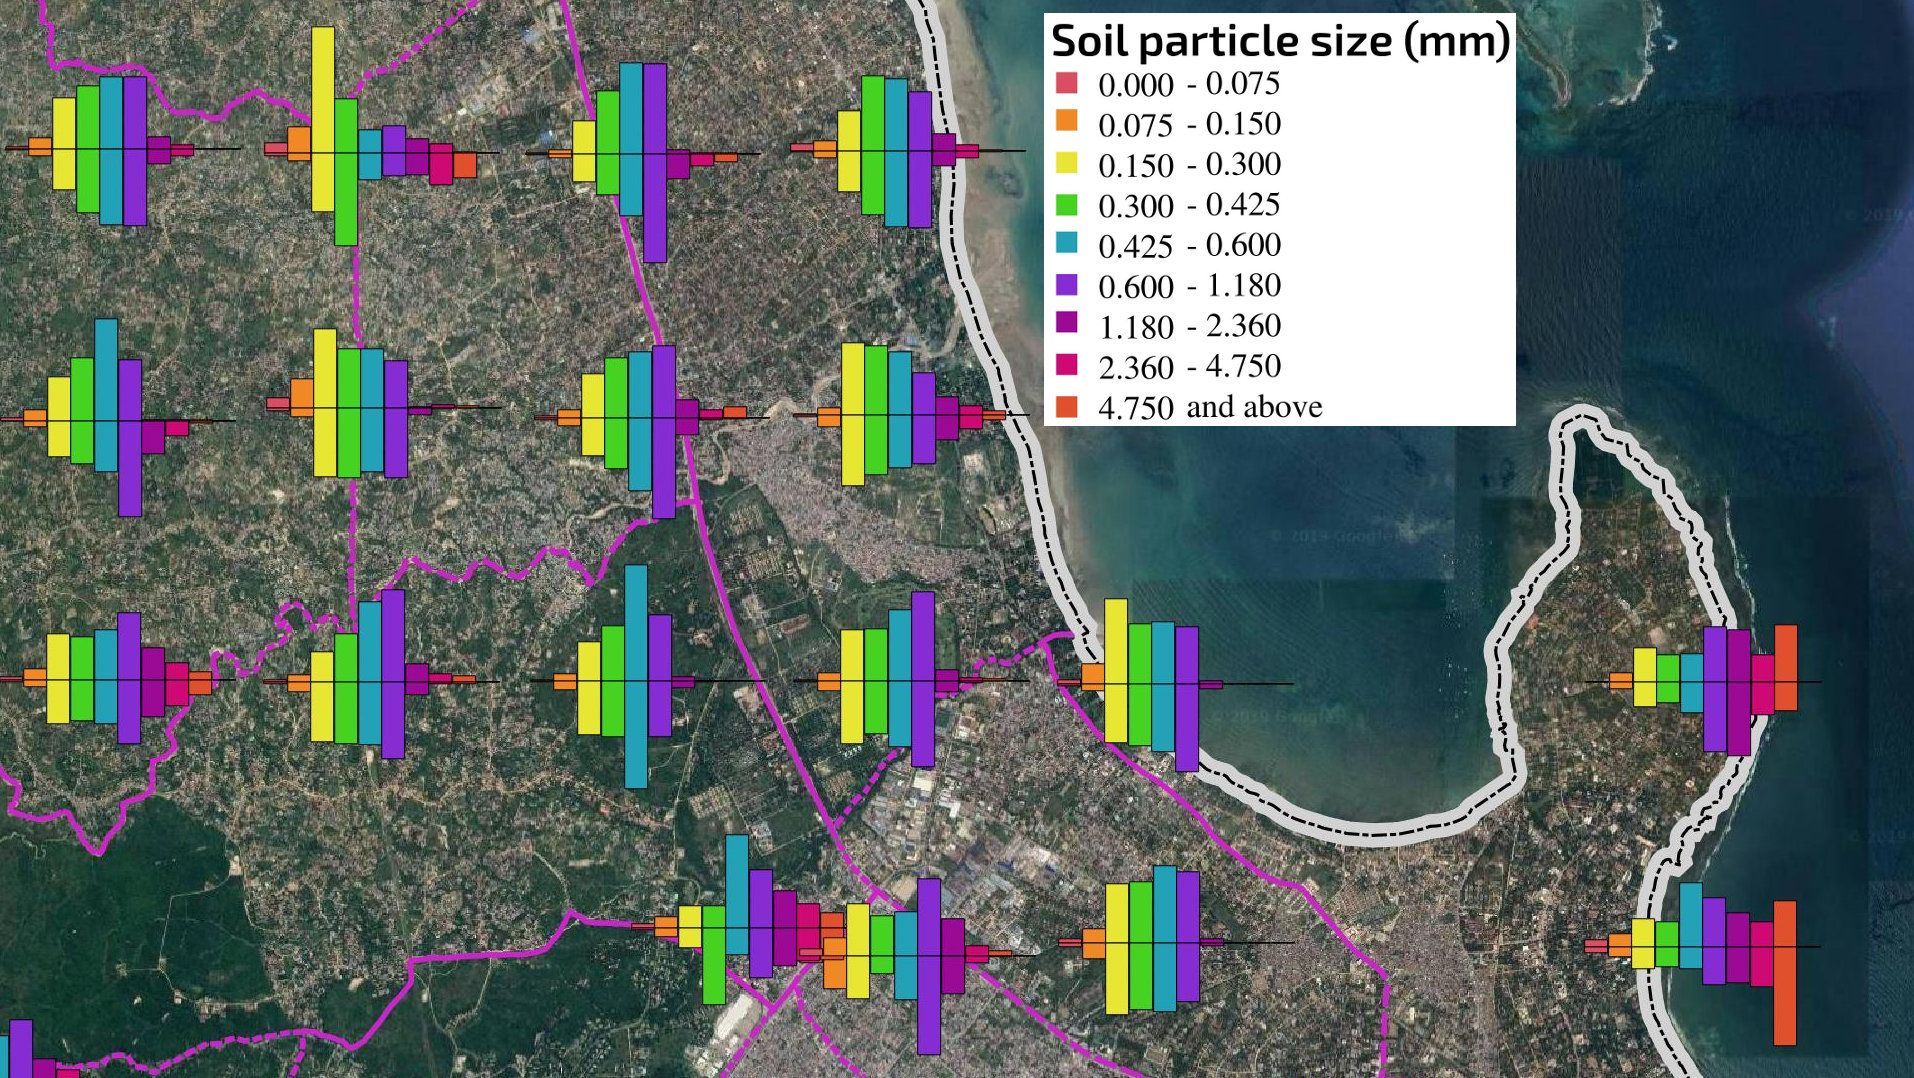
\includegraphics[width=1\textwidth]{soil_map_detail_peninsula_with_legend}
\end{figure}

\subsubsection{Statistics}
731 soil sample points created using a 2 km grid. 643 points sampled and sieved; 88 sample points were either inaccessible or hard to collect sample e.g. paved areas, military base.

\subsubsection{Data Visualization}

\subsubsection{Use Case}
This data is primarily intended for use with erosion modeling. For users not equipped with erosion modeling skills and toolkits, and for sharing the results with the public, a visual map has been prepared that gives a good first impression of the characteristics of the soil.
The resulting dataset, a geo-referenced set of soil profiles, has been published as \href{https://geonode.uhurulabs.org/layers/geonode3A_2019_02_26_dar_soil_sampling_final_results_v1}{open data}\footnote{\url{https://geonode.uhurulabs.org/layers/geonode3A_2019_02_26_dar_soil_sampling_final_results_v1}}.

\subsubsection{Data Gap}
88 points were not collected because they were inaccessible

\subsubsection{Lesson Learned}

\newpage
\subsection{Trash Mapping in Formal Settlement (Green WastePro Limited)}
Green WastePro Limited is a private company specialized in waste management with the aim to offer eco-friendly solutions in cleaning and waste management. They are mostly operate in formal settlements. The company needed digital methodology to obtain clients’ information including locations, clients contacts etc, so they can track clients and provide services accordingly.

\newpage
\subsection{Trash Mapping in Informal Settlement (Joshemi Company Limited)}

\newpage
\subsection{Dar es Salaam Trash Data}

A collaboration between Nipe Fagio (“give me the broom” in Swahili), a civil society organisation founded in 2013 and Ramani Huria that joined forces and mapped trash sites in Dar es Salaam. The trash mapping initiative was part and parcel of the large Let’s-Do-It-World campaign, a civic-led mass movement to clean up countries.
The mapped data helped to identify location of the areas with poorly managed waste materials, type and size of waste and clean up methods. This process helped ease cleaning the city on September 15th, 2018, a celebration of the world clean up day.

\subsubsection{Data Collection Methodology}
Using OpenDataKit to collect trash points in the city and filling out the survey on the type of waste (debris, glass, metal), and the size of trash (hand full, bag full, truckload, cart etc) to ease cleaning process.

Before field work, introduction letters were sent to ward officers so they can be informed and for mappers security in case there is any assistance needed from the ward office.

\subsubsection{Quality Assurance}
Some categories such as handful and bagful were far too small to be collected and sometimes confused the mappers therefore a decision to remove these points had to be made which dropped the number of points to approximately 9,000.

\newpage
\subsection{Community Flood Response Mapping}

\newpage
\section{Annexes}

\end{document}